\documentclass[aspectratio=169,12pt]{beamer}
\usepackage[utf8]{inputenc}
\usepackage[spanish, es-nodecimaldot]{babel}
%\usepackage{icomma} % Use dot as decimal separator
\usepackage{booktabs} % For better-looking tables
\usepackage{wrapfig}
%\usepackage{siunitx}

\usepackage{multicol}
\usepackage{mathtools}

\usepackage[normalem]{ulem}

\pagestyle{empty}

\usepackage{pgf,tikz}
\usepackage{pgfplots}
\usetikzlibrary{matrix}
\usetikzlibrary{arrows}

%\usepackage{wrapfig}
\mode<presentation>
\usefonttheme{professionalfonts}
\usetheme{Darmstadt}
\usecolortheme{orchid}
\useoutertheme{default}
\setbeamertemplate{headline}{}

\renewcommand{\baselinestretch}{1.1}

%gets rid of bottom navigation bars
\setbeamertemplate{footline}[page number]

%gets rid of navigation symbols
\setbeamertemplate{navigation symbols}{}

%\frameframe{none} % No default frame

%\setlength{\framewidth}{8.7in} \setlength{\frameheight}{7.2in}

\parindent 0pt
\setlength{\parskip} {1ex plus 0.5ex minus 0.2ex}


%\usepackage[bbgreekl]{mathbbol}
\usepackage{amsfonts}

%\DeclareSymbolFontAlphabet{\mathbb}{AMSb}
%\DeclareSymbolFontAlphabet{\mathbbl}{bbold}

\newcommand{\Sym}{{\mathcal S}}
\DeclareMathOperator{\Aut}{Aut}
\DeclareMathOperator{\Tr}{Tr}
\DeclareMathOperator{\trace}{Trace}
\DeclareMathOperator{\range}{range}
\DeclareMathOperator{\rank}{rank}

\usepackage{breqn}
\usepackage{multicol}
\usepackage{colortbl}
\usepackage{lmodern}
\usepackage{tabularx}
\usepackage{multirow}
\usepackage{amssymb}
\usepackage{amsmath}
\usepackage{stmaryrd}
\usepackage{color}
\usepackage{graphicx}
\graphicspath{ {img/} }
\usepackage{hyperref}

\input{epsf}
\title{Introducción}
\author{}

\DeclareMathOperator{\Hom}{Hom}
\DeclareMathOperator{\sing}{sing}

\DeclareMathOperator{\chara}{char}
\DeclareMathOperator{\Jacob}{Jacob}
\DeclareMathOperator{\Sing}{Sing}
\newcommand{\fracNoLine}[2]{\genfrac{}{}{}{0pt}{#1}{#2}}

%\beamerdefaultoverlayspecification{<+->}

\usepackage{listings,xcolor,bm}


\definecolor{mygreen}{rgb}{0,0.6,0}
\definecolor{mygray}{rgb}{0.5,0.5,0.5}
\definecolor{mymauve}{rgb}{0.58,0,0.82}
\lstset{
  backgroundcolor=\color{white},   % choose the background color; you must add
  basicstyle=\small\ttfamily,      % the size of the fonts that are used for the code
  breakatwhitespace=false,         % sets if automatic breaks should only happen at whitespace
  breaklines=true,                 % sets automatic line breaking
  captionpos=b,                    % sets the caption-position to bottom
  commentstyle=\color{mygreen},    % comment style
  deletekeywords={...},            % if you want to delete keywords from the given language
  escapeinside={\%*}{*)},          % if you want to add LaTeX within your code
  extendedchars=true,              % lets you use non-ASCII characters; for 8-bits encodings only, does not work with UTF-8
  firstnumber=1,                % start line enumeration with line 1000
  frame=single,	                   % adds a frame around the code
  keepspaces=true,                 % keeps spaces in text, useful for keeping indentation of code (possibly needs columns=flexible)
  keywordstyle=\color{blue},       % keyword style
  language=Python,                 % the language of the code
  morekeywords={*,...},            % if you want to add more keywords to the set
  numbers=left,                    % where to put the line-numbers; possible values are (none, left, right)
  numbersep=5pt,                   % how far the line-numbers are from the code
  numberstyle=\tiny\color{mygray}, % the style that is used for the line-numbers
  rulecolor=\color{black},         % if not set, the frame-color may be changed on line-breaks within not-black text (e.g. comments (green here))
  showspaces=false,                % show spaces everywhere adding particular underscores; it overrides 'showstringspaces'
  showstringspaces=false,          % underline spaces within strings only
  showtabs=false,                  % show tabs within strings adding particular underscores
  stepnumber=5,                    % the step between two line-numbers. If it's 1, each line will be numbered
  stringstyle=\color{mymauve},     % string literal style
  tabsize=4,	                   % sets default tabsize to 2 spaces
  title=\lstname                   % show the filename of files included with \lstinputlisting; also try caption instead of title
}

\begin{document}

\newtheorem{prop}{Proposici\'on}
\newtheorem{algo}[prop]{Algorithm}
\newtheorem{teor}[prop]{Theorem}
\newtheorem{lema}[prop]{Lemma}
\newtheorem{coro}[prop]{Corollary}
\newtheorem{defi}[prop]{Definition}

\newcommand{\ideal}[1]{{\left\langle{#1}\right\rangle}}
\newcommand{\demo}{\textbf {Demostraci\'on. }}
\newcommand{\obse}{\textbf {Observaci\'on. }}
\newcommand{\Input}{\textbf {Input: }}
\newcommand{\Output}{\textbf {Output: }}
\newcommand{\Examp}{\textbf {Ejemplo }}
\newcommand{\Examps}{\textbf {Ejemplos }}

\newcommand{\kk}{{\mathbbl k}}
\newcommand{\V}{{\mathbf V}}
\newcommand{\I}{{\mathbf I}}
\newcommand{\PP}{{\tilde P}}
\newcommand{\QQ}{{\tilde Q}}

\newcommand{\F}{{\mathbb F}}
\newcommand{\Q}{{\mathbb Q}}
\newcommand{\N}{{\mathbb N}}
\newcommand{\R}{{\mathbb R}}
\newcommand{\Z}{{\mathbb Z}}
\newcommand{\CC}{{\mathbb C}}
\newcommand{\eLL}{{\mathcal L}}



\newcommand{\MinAss}{\textrm {MinAss}}
\newcommand{\Ass}{\textrm {Ass}}
\newcommand{\mcm}{\textrm {mcm}}
\newcommand{\mcd}{\textrm {mcd}}
%\newcommand{\mod}{\textrm { mod }}
\newcommand{\lt}{\textrm {lt}}
\newcommand{\Lt}{\textrm {Lt}}
\newcommand{\lp}{\textrm {lp}}
\newcommand{\lc}{\textrm {lc}}
\newcommand{\lm}{\textrm {lm}}
\newcommand{\barra}{\ /\ }
\newcommand{\multideg}{\textrm {multideg}}

\newcommand{\sep}{\textrm {sep}}
\newcommand{\Syz}{\textrm {Syz}}
\newcommand{\n}{\~n}
\newcommand{\cG}{\textrm {cG}}
\newcommand{\dG}{\textrm {dG}}
\newcommand{\nG}{\textrm {nG}}
\newcommand{\CE}{\textrm {CE}}
\newcommand{\CG}{\textrm {CG}}
\newcommand{\CF}{\textrm {CF}}
\newcommand{\DG}{\textrm {DG}}
\renewcommand{\NG}{\textrm {NG}}

\newcommand{\p}{{\boldsymbol{p}}}
\newcommand{\q}{{\boldsymbol{q}}}

\newcommand{\X}{{\boldsymbol{X}}}
\newcommand{\x}{{\boldsymbol{x}}}
\renewcommand{\u}{{\boldsymbol{u}}}
\renewcommand{\t}{{\boldsymbol{t}}}
\renewcommand{\a}{{\boldsymbol{a}}}
\renewcommand{\b}{{\boldsymbol{b}}}
\renewcommand{\c}{{\boldsymbol{c}}}

%Titulos en espa�ol
%\renewcommand{\chaptername}{Cap\'{\i}tulo}
%\renewcommand{\bibname}{Bibliograf\'{\i}a}

\newcommand{\kring}{\kk[\x]}
\newcommand{\kRing}{\kk[X]}
\newcommand{\qring}{\Q[\x]}

%\renewcommand\itemindent{-10pt}
%\renewcommand{\theenumi}{\arabic{enumi}}
%\renewcommand{\labelenumi}{\Alph{enumi}}

\definecolor{issac}{rgb}{1.00,0.00,0.00}
%------------------------------------------------------------------

\begin{frame}

 \begin{center}

\Large\textbf{Laboratorio de Datos} \\
\large\textbf{Entrenamiento y testeo}
%\vspace{0.5cm}

% \textit{Santiago Laplagne} \\
%slaplagn@dm.uba.ar \\


%\vspace{0.5cm}
%{\small Trabajo en progreso en conjunto con \emph{Jose Capco} (Universit\"at Innsbruck) y \emph{Claus Scheiderer} %(Universit\"at Konstanz).} \\

\vspace{1cm}
Primer Cuatrimestre 2024 \\ Turnos tarde y noche

\vspace{1cm}


 {\small Facultad de Ciencias Exactas y Naturales, UBA}
 \end{center}


\end{frame}

%------------------------------------------------------------------

\begin{frame}
\frametitle{?`C\'omo elegir entre distintos modelos?}

Toda tarea de «aprendizaje automático», «machine learning» o «inteligencia artificial»,
consiste en:
\begin{enumerate}
\item Tomar un problema relevante del mundo material.
\item Elegir un modelo matemático que lo represente. El modelo en general va a depender de ciertos parámetros $\beta_1, \dots, \beta_s$.
Por ejemplo en un modelo de regresión lineal, estos parámatros son los coeficientes de cada variable.
\item Definir una forma de medir qu\'e tan bueno es un modelo, en relación a la realidad (vía los datos disponibles).
Esto suele hacerse mediante una \emph{función de pérdida}.
\item $\dots$
\end{enumerate}
\end{frame}

%------------------------------------------------------------------

\begin{frame}
\frametitle{?`C\'omo elegir entre distintos modelos?}

\textbf{Función de pérdida:} Si fijamos los parámetros de nuestro modelo $\beta_1, \dots, \beta_s$ y aplicamos el modelo resultante a un conjunto de datos $X$, la función de pérdida mide cuánto ``perdemos'' utilizando el modelo en lugar de los datos reales.

En regresión lineal, la función de pérdida más común es el \emph{error cuadrático medio (MSE)}.

Vamos a llamar $L(\beta \mid X)$ a la función de pérdida para un conjunto de par\'ametros $\beta = (\beta_1, \dots, \beta_s)$ y un conjunto de datos $X$.

\end{frame}


%------------------------------------------------------------------

\begin{frame}
\frametitle{?`C\'omo elegir entre distintos modelos?}

Toda tarea de «aprendizaje automático», «machine learning» o «inteligencia artificial»,
consiste en:
\begin{enumerate}
\item Tomar un problema relevante del mundo material.
\item Elegir un modelo matemático que lo represente. El modelo en general va a depender de ciertos parámetros $\beta_1, \dots, \beta_s$.
Por ejemplo en un modelo de regresión lineal, estos parámatros son los coeficientes de cada variable.
\item Definir una una \emph{función de pérdida} $L(\beta \mid X)$.
\item ``Aprender'' los coeficientes $\beta_1, \dots, \beta_s$. Es decir, encontrar valores $\beta_1, \dots, \beta_s$ que minimicen la pérdida.
\end{enumerate}
\end{frame}

%------------------------------------------------------------------

\begin{frame}
\frametitle{Nivel 1: Entrenar y evaluar sobre todo el conjunto de datos}

Como primer acercamiento, entrenamos nuestros modelos con un conjunto de datos $X$ y evaluamos la perfomance sobre \emph{los mismos datos $X$}.

En este contexto, si un modelo $M_1$ es \emph{más complejo} que un modelo $M_0$ (es decir tiene más variables o parámetros), entonces necesariamente el valor de la función de pérdida será menor o igual.
\end{frame}

%------------------------------------------------------------------

\begin{frame}
\frametitle{Nivel 1: Entrenar y evaluar sobre todo el conjunto de datos}

Ejemplo:
\begin{itemize}
\item $M_0: \text{gastos mensuales} \sim b_0 + b_1 \cdot \text{sueldo} + b_2 \cdot \text{cantidad de hijos}$
\item $M_1: \text{gastos mensuales} \sim b_0 + b_1 \cdot \text{sueldo} + b_2 \cdot \text{cantidad de hijos} + b_3 \cdot \text{altura}$
\end{itemize}

El modelo $M_1$ es m\'as complejo que $M_0$. Podemos ver a $M_0$ como un caso particular de $M_1$ tomando $b_3 = 0$.

El valor mínimo de pérdida de $M_1$ es menor o igual que el valor mínimo de pérdida de $M_0$:
$$
L_{M_1}(\beta_0^*,\beta_1^*,\beta_2^*,\beta_3^* \mid X) \le L_{M_0}(\beta_0^*,\beta_1^*,\beta_2^* \mid X)
$$

\end{frame}


%------------------------------------------------------------------

\begin{frame}
\frametitle{Nivel 1: Entrenar y evaluar sobre todo el conjunto de datos}

En este esquema, un valor de pérdida menor no nos asegura que el modelo $M_1$ sea mejor que $M_0$ (tenga mejor capacidad predictiva).

Que un modelo alcance un error muy pequeño durante el entrenamiento, puede ser tanto mérito propio del modelo como un síntoma de una excesiva parametrización, que le permite ``interpolar'' o ``memorizar'' los datos.

\textbf{Ejemplo:} Si tenemos $n$ observaciones y tomamos un polinomio de grado $n-1$ o un modelo con $n$ variables (independientes), vamos a poder obtener un modelo exacto, la pérdida será 0.

\end{frame}

%------------------------------------------------------------------

\begin{frame}
\frametitle{Nivel 2: Separar en conjuntos de entrenamiento («train») y prueba («test»)}

Para evitar el \emph{sobreajuste} (overfitting) de los modelos, es habitual dividir el conjunto
de datos en dos partes mutuamente excluyentes (y conjuntamente exhaustivas, ¡nada
se tira!).

Entrenaremos cada modelo con los mismos datos de train para obtener los $\beta$
óptimos, pero seleccionaremos como ``mejor'' a aquel modelo que minimice la pérdida  sobre el conjunto de test.


\end{frame}

%------------------------------------------------------------------

\begin{frame}
\frametitle{Nivel 3: Split entrenamiento - validación - prueba}

Como antes argumentamos que el modelo que minimiza el error de entrenamiento
puede estar sobreajustándose a los datos, es igualmente posible que aquél que minimiza el error de prueba esté sobreajustándose a los datos de prueba: al fin y al cabo, así fue como definimos nuestra regla de selección (minimizar el error de prueba).
\end{frame}

%------------------------------------------------------------------

\begin{frame}
\frametitle{Nivel 3: Split entrenamiento - validación - prueba}

Para evitar este problema, se suele dividir el conjunto de datos en tres partes: entrenamiento, validación y test:
\begin{enumerate}
\item Entrenamos los modelos minimizando $L$ en $X_{\text{train}}$ (los datos de entrenamiento).
\item Una vez entrenados los modelo, medimo la pérdida $L$ en $X_{\text{val}}$ y seleccionamos el modelo con menor pérdida.
\item Evaluamos su performance ``en el mundo real'' con $L$ en $X_{\text{test}}$.
\end{enumerate}

\end{frame}

%------------------------------------------------------------------

\begin{frame}
\frametitle{Nivel 4: Validación Cruzada en $k$ Pliegos (``K-fold CV'')}

En un esquema tripartito «train-val-test», el error de test sólo sirve para reporte, y
achica el tamaño efectivo de la muestra. 

Más aún, como hay un único conjunto de
test, y todo el proceso está atravesado por ruido estocástico, la selección de modelos
sigue teniendo un fuerte componente de azar.

Para evitar posibles sesgos en la selección de los conjuntos de entranamiento y validación, resulta conveniente realizar varias repeticiones del experimento con distintos conjuntos de datos. ¿Pero de dónde sacamos los datos para ello?

¡Pues los reutilizamos!

\end{frame}


%------------------------------------------------------------------

\begin{frame}
\frametitle{Nivel 4: Validación Cruzada en $k$ Pliegos (``K-fold CV'')}


En validación cruzada de $k$ pliegos (``k-fold cross-validation''), dividimos primero el conjunto de datos sólo en
train y test. 

Luego, partimos train en $k$ partes iguales, que se rotarán el papel de validaci\'on: entrenamos y
evaluamos el modelo $k$ veces, cada vez dejando uno distinto de los $k$ pliegos como \emph{val} y el resto para \emph{train}.

\begin{center}
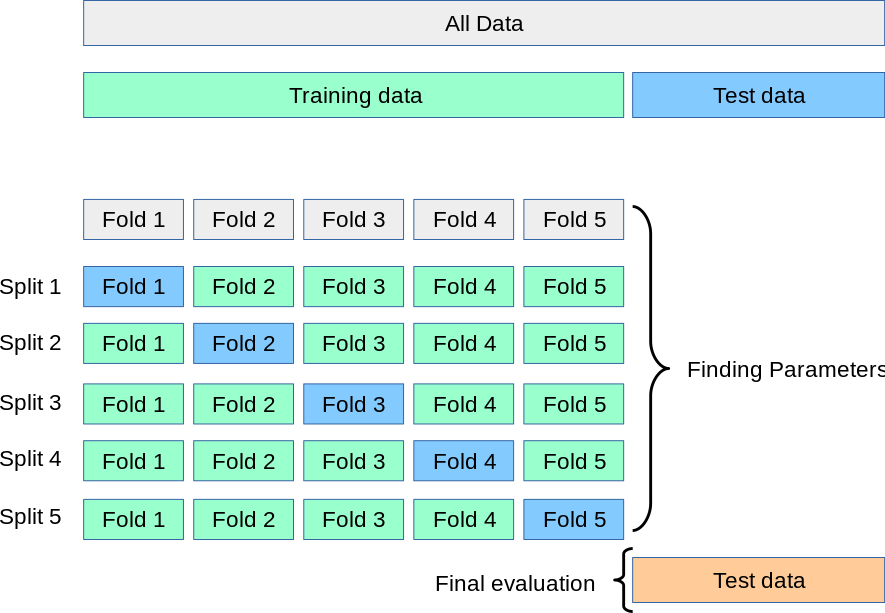
\includegraphics[scale=0.2]{clase10-grid_search_cross_validation.png}
\end{center}


\end{frame}

\end{document}
